\chapter{Suport teoretic}
\label{chap:suport-teoretic}

\section{Apicultură digitală și trasabilitatea lucrărilor}

Digitalizarea apiculturii se înscrie într-o direcție mai amplă, cunoscută în literatura de specialitate sub numele de \emph{apicultură de precizie} (\emph{Precision Beekeeping}), care urmărește gestionarea fiecărei familii de albine pe baza datelor colectate, pentru a reduce pierderile și a îmbunătăți deciziile apicultorului \cite{zacepins2015precision}. Lucrările din acest domeniu arată că monitorizarea continuă și înregistrarea sistematică a stării coloniilor oferă informații utile pentru intervenții la timp \cite{meikle2015monitoring}. Totuși, digitalizarea apiculturii nu înseamnă doar mutarea unei agende pe telefon. O aplicație utilă trebuie să transforme observațiile de teren în date care pot fi regăsite, comparate și interpretate. În apicultură, aceeași familie de albine trece prin stări diferite de-a lungul sezonului: dezvoltare de primăvară, cules, roire, tratamente, pregătire pentru iernare și perioade de repaus. Pentru a înțelege corect starea unui stup, apicultorul are nevoie de continuitate între observații.

Conceptul de trasabilitate este relevant în acest context. Trasabilitatea presupune păstrarea unui istoric coerent al evenimentelor care afectează un obiect urmărit. În BeeSmart, obiectul urmărit poate fi stupina, stupul sau inspecția. Pentru un stup, istoricul poate include date despre matcă, rame, puiet, rezerve, tratamente, extracții, fotografii și analize AI. Dacă aceste informații sunt introduse consecvent, aplicația poate oferi o imagine mai clară decât o notă izolată.

Trasabilitatea este importantă și pentru decizii practice. De exemplu, un tratament antivarroa trebuie urmărit în timp, nu doar notat în ziua aplicării. O scădere a puietului trebuie comparată cu inspecțiile anterioare, nu interpretată fără context. O extracție trebuie corelată cu perioada de cules și cu starea familiei. În lipsa unui sistem digital, aceste corelații depind de memoria utilizatorului sau de calitatea agendei scrise.

BeeSmart urmărește să ofere această structură prin entități clare: stupine, stupi, inspecții, tratamente, extracții și task-uri. Fiecare entitate contribuie la istoricul apicol.

\section{Datele apicole ca date sezoniere}

Un aspect specific apiculturii este sezonalitatea. Datele apicole nu sunt uniforme pe tot parcursul anului. Primăvara, accentul cade pe dezvoltarea familiei, existența mătcii și extinderea cuibului. Vara, atenția se mută spre cules, spațiu, prevenirea roirii și extracții. Toamna, tratamentele și pregătirea rezervelor devin prioritare. Iarna, activitatea de inspecție este redusă, dar istoricul rămâne util pentru planificarea sezonului următor.

Din perspectiva unei aplicații, această sezonalitate înseamnă că datele trebuie păstrate în timp și prezentate comparativ. O valoare precum numărul de rame cu puiet este utilă doar dacă poate fi raportată la data inspecției și la starea anterioară a stupului. De aceea, BeeSmart nu se limitează la o listă curentă de stupi. Aplicația păstrează istoricul inspecțiilor și poate folosi rezultatele AI pentru a construi tendințe.

Un alt efect al sezonalității este faptul că anumite date sunt importante doar în contexte precise. Vremea contează în mod special la inspecții, zbor și cules. Tratamentele au ferestre de aplicare. Extracțiile sunt relevante în raport cu culesul și cu rezervele rămase în stup. Task-urile ajută la planificarea acestor intervenții, dar ele trebuie legate de stupină sau stup pentru a nu deveni simple memento-uri generale.

\section{Inspecția ca act central în managementul apicol}

Inspecția este una dintre operațiile centrale ale managementului apicol. În timpul unei inspecții, apicultorul observă direct starea familiei și notează informații despre cuib, hrană, matcă, puiet și eventuale probleme. În BeeSmart, formularul de inspecție reflectă aceste elemente prin câmpuri precum temperatura, numărul total de rame, rame cu puiet, rame cu miere, rame cu polen, prezența mătcii, prezența ouălor și a larvelor.

O inspecție are valoare imediată, dar și valoare istorică. Valoarea imediată apare în decizia de moment: trebuie adăugată hrană, trebuie căutată matca, trebuie verificată roirea, trebuie aplicat tratament. Valoarea istorică apare când inspecția este comparată cu altele. Dacă un stup avea puiet compact la începutul lunii și apoi scade brusc, aplicația poate ajuta utilizatorul să observe schimbarea. Dacă tratamentele și extracțiile sunt păstrate în același sistem, datele devin mai ușor de corelat.

În proiectarea unei aplicații mobile, formularul de inspecție trebuie să fie suficient de detaliat, dar nu excesiv de încărcat. Dacă formularul este prea simplu, nu colectează date utile. Dacă este prea lung, utilizatorul nu îl va completa în teren. BeeSmart încearcă să echilibreze aceste cerințe prin câmpuri structurate, fotografii, introducere vocală și valori care pot fi completate rapid.

\section{Rolul fotografiilor de rame}

Fotografia unei rame adaugă un strat vizual la inspecție. Ea poate surprinde detalii pe care utilizatorul nu le notează complet în momentul inspecției. Poate fi revăzută ulterior, comparată cu alte imagini și folosită pentru analiză automată. În aplicații apicole, fotografia nu trebuie privită doar ca atașament decorativ, ci ca o formă de date.

Totuși, o fotografie brută are limite. Două imagini pot fi greu de comparat dacă sunt făcute la distanțe diferite, în lumină diferită sau din unghiuri diferite. De aceea, analiza automată urmărește să transforme imaginea într-o reprezentare numerică: câte celule au fost detectate, câte aparțin fiecărei clase și ce indicatori pot fi calculați din aceste valori.

În BeeSmart, fotografia este introdusă din formularul de inspecție și este trimisă către backend pentru analiză. Clientul Android nu rulează modelul DeepBee direct. Această decizie are avantajul de a păstra aplicația mobilă mai ușoară și de a centraliza procesarea AI într-un serviciu specializat. Dezavantajul este că analiza necesită conexiune la backend și la serviciul AI. Prin urmare, fotografia poate exista ca parte a inspecției offline, dar analiza automată depinde de infrastructura server.

În implementarea curentă, fotografia are două reprezentări practice. Prima este fișierul procesat păstrat pentru inspecție, la o calitate potrivită pentru arhivare și revizualizare. A doua este versiunea trimisă către AI, redimensionată la maximum 1536 px și comprimată înainte de codarea Base64. Această separare a redus payload-ul transmis de pe telefon, fără să elimine fotografia din istoricul inspecției.

\section{Sisteme offline-first}

Un sistem offline-first este proiectat astfel încât absența temporară a conexiunii să nu blocheze complet utilizarea aplicației. Într-un model clasic, clientul trimite cereri la server și așteaptă răspunsul pentru a considera operația finalizată. Într-un model offline-first, clientul păstrează o copie locală a datelor și poate înregistra operații care vor fi sincronizate ulterior.

Pentru BeeSmart, această strategie este justificată de mediul de utilizare. Stupinele pot fi amplasate în zone cu semnal slab, iar apicultorul nu ar trebui să piardă date doar pentru că serverul nu este accesibil în acel moment. Când utilizatorul creează o inspecție offline, aplicația trebuie să îi ofere un răspuns imediat și să salveze local operația. Când conexiunea revine, aplicația trimite datele la server.

Din punct de vedere teoretic, offline-first introduce problema consistenței. Datele locale pot fi temporar diferite de cele de pe server. Această stare este acceptabilă dacă aplicația știe ce operații sunt în așteptare și le poate sincroniza într-o ordine corectă. În BeeSmart, coada de sincronizare este soluția pentru această problemă. Ea reține operațiile și permite procesarea lor când condițiile de rețea sunt favorabile.

\section{Consistență eventuală și dependențe între entități}

Consistența eventuală înseamnă că sistemul poate avea stări temporar diferite în componente diferite, dar urmărește ca acestea să ajungă la aceeași stare după sincronizare \cite{vogelsEventualConsistency}. Într-o aplicație mobilă offline, această idee apare natural. Telefonul poate conține date noi pe care serverul nu le-a primit încă. După sincronizare, serverul primește datele, iar clientul actualizează identificatorii și statusurile locale.

În BeeSmart, dependențele dintre entități fac sincronizarea mai complexă. O stupină poate exista fără stupi, dar un stup are nevoie de o stupină. O inspecție are nevoie de un stup. O fotografie are nevoie de o inspecție. Dacă utilizatorul creează offline toate aceste elemente, aplicația trebuie să păstreze relațiile locale și apoi să le transforme în relații de server. Aceasta este problema rezolvării identificatorilor.

De exemplu, o stupină creată offline primește un id local. Stupul creat în acea stupină referă id-ul local al stupinei. Când stupina este sincronizată, serverul returnează un id real. Abia apoi stupul poate fi trimis la server cu id-ul corect al stupinei. Același principiu se aplică în lanțul de dependențe prezentat în figura~\ref{fig:ordine-sincronizare-offline}: de la stupină, către stup, apoi către task-uri, tratamente, extracții, inspecții și, în final, fotografii. Dacă aplicația ar încerca să trimită un element copil înainte ca părintele să fie sincronizat, backend-ul nu ar putea găsi referința. De aceea, procesarea în ordinea dependențelor nu este un detaliu de implementare, ci o cerință teoretică a modelului offline-first.

\section{Securitatea datelor și ownership}

BeeSmart gestionează date care aparțin unui utilizator: stupine, stupi, inspecții, fotografii și analize. Chiar dacă aceste date nu sunt la fel de sensibile ca datele medicale sau financiare, ele pot avea valoare economică și profesională. Un apicultor nu ar trebui să poată accesa datele altuia, iar pierderea sau amestecarea datelor ar afecta încrederea în aplicație.

Autentificarea prin JWT rezolvă doar o parte a problemei. Un token valid arată că utilizatorul este autentificat, dar nu demonstrează automat că are dreptul asupra fiecărei resurse cerute. De aceea, backend-ul trebuie să verifice ownership-ul la nivel de servicii și repository-uri. În BeeSmart, controllerele extrag id-ul utilizatorului din token, iar serviciile verifică dacă resursele aparțin acelui utilizator înainte de mutații.

Pe client, securitatea se leagă și de starea locală. Dacă utilizatorul se deloghează sau se autentifică alt cont, aplicația trebuie să evite afișarea datelor vechi. De asemenea, token-urile trebuie gestionate cu atenție, iar refresh-ul nu trebuie să creeze bucle de cereri. Aceste aspecte sunt relevante pentru orice aplicație offline-first, deoarece datele persistă pe dispozitiv chiar și după întreruperi de rețea.

\section{DeepBee ca punct de plecare pentru analiza ramelor}

Componenta teoretică principală a analizei automate este articolul \enquote{Automatic detection and classification of honey bee comb cells using deep learning} \cite{deepbeeArticle}. Articolul prezintă o metodă pentru detectarea și clasificarea celulelor din imagini de fagure. Scopul unei astfel de metode este extragerea automată a unor informații care, altfel, ar necesita observare manuală atentă.

DeepBee împarte problema în mai multe etape. Mai întâi, celulele trebuie detectate în imagine. Apoi, regiunile detectate trebuie filtrate pentru a reduce detecțiile false. În final, fiecare celulă detectată trebuie clasificată într-una dintre clasele relevante. Această împărțire este logică: înainte de a decide ce conține o celulă, sistemul trebuie să știe unde se află celula.

Pentru BeeSmart, articolul DeepBee oferă baza conceptuală pentru integrarea AI. Aplicația nu revendică modelul ca fiind original, ci folosește ideea de analiză automată a celulelor pentru a completa inspecțiile apicole. În acest fel, contribuția lucrării este aplicativă: modelul este introdus într-un flux Android-backend-AI, iar rezultatul devine parte a istoricului stupului.

Integrarea a pornit de la implementarea de referință publicată de autori \cite{deepbeeSource}, iar nucleul algoritmic a fost păstrat fidel: aceleași modele \path{segmentation.h5} și \path{classification.h5}, aceeași ordine a claselor la decodarea predicțiilor, aceiași parametri ai transformatei Hough (inclusiv formula razei dominante pentru distanța minimă dintre centre), aceeași pregătire a imaginii pe canalul roșu cu egalizare locală de contrast și filtrare bilaterală și aceeași decupare proporțională cu raza, redimensionată la 224 x 224 pixeli înainte de clasificare. Fidelitatea față de varianta originală este importantă pentru corectitudine: modelul a fost antrenat pe un anumit mod de pregătire a datelor, iar o abatere de la acesta ar degrada predicțiile fără ca formatul răspunsului să pară greșit.

În același timp, codul de referință este o aplicație desktop care procesează loturi de fotografii din foldere locale și presupune resurse de calcul generoase. Pentru ca metoda să poată fi apelată dintr-o aplicație mobilă, în cadrul lucrării au fost necesare mai multe adaptări:
\begin{itemize}
	\item transformarea pipeline-ului într-un microserviciu Flask cu rutele \path{/analyze} și \path{/health}, cu intrare Base64 și răspuns JSON; inferența folosește o singură sesiune TensorFlow partajată și este serializată printr-un mecanism de blocare, deoarece combinația Keras 2 / TensorFlow 1 nu este thread-safe într-un server web;
	\item înlocuirea reconstrucției măștii de segmentare la rezoluția fixă de 6000 x 4000 pixeli cu o limită configurabilă a muchiei maxime (implicit 2200 px) și cu o grilă de patch-uri calculată dinamic pe dimensiunile reale ale imaginii, masca rezultată fiind scalată înapoi peste imaginea analizată; această schimbare face inferența stabilă pe containerul cu resurse limitate din Azure;
	\item restructurarea clasificării astfel încât decupajele de 224 x 224 pixeli să fie extrase și clasificate în loturi, fără a păstra simultan în memorie toate regiunile unei rame dense, așa cum procedează varianta originală;
	\item reinterpretarea scorului de încredere: în codul original, pragul foarte ridicat de 0,9995 marchează doar celulele potrivite pentru reantrenarea modelului, în timp ce în BeeSmart un prag de 0,60 pe celulă și un raport maxim de 75\% predicții slabe decid dacă întreaga analiză este declarată incertă.
\end{itemize}

Pe lângă aceste adaptări, serviciul adaugă elemente care nu există în implementarea de referință: criteriile de calitate aplicate înainte de model (dimensiune minimă, claritate, luminozitate, contrast), statusurile de răspuns dedicate imaginilor nepotrivite, pragul minim de celule detectate și metadatele de calitate atașate fiecărui răspuns (numărul de celule detectate și clasificate, încrederea medie și timpii pe etape). Aceste extensii sunt detaliate în secțiunile următoare ale capitolului. În sens invers, componentele desktop ale proiectului original — vizualizarea interactivă, corectarea manuală a predicțiilor, exportul tabelar și reantrenarea — nu au fost preluate, deoarece nu se potrivesc unui serviciu apelat automat din aplicație. Ca format de răspuns, serviciul întoarce distribuția celulelor pe clase împreună cu metadatele de calitate, adică exact forma de care au nevoie indicatorii derivați și statisticile longitudinale construite peste analiză în aplicație.

\section{Cele șapte clase de celule}

Modelul DeepBee urmărește clasificarea celulelor în șapte clase: ouă, larve, puiet căpăcit, polen, nectar, miere și alte celule \cite{deepbeeArticle}. Aceste clase sunt relevante deoarece descriu atât activitatea de reproducere a coloniei, cât și rezervele de hrană. Ouăle și larvele indică prezența unei ponte recente, puietul căpăcit indică dezvoltarea în curs, iar mierea, nectarul și polenul descriu resursele disponibile.

În serviciul BeeSmart, ieșirea modelului este interpretată în ordinea folosită de repository-ul DeepBee: \path{Capped}, \path{Eggs}, \path{Honey}, \path{Larves}, \path{Nectar}, \path{Other} și \path{Pollen}. Această ordine este importantă deoarece vectorul de probabilități produs de rețeaua neuronală nu conține etichete text, ci doar poziții numerice. Dacă pozițiile ar fi asociate greșit, rezultatul ar părea valid ca format, dar ar descrie categorii biologice eronate. În interfața pentru utilizator, rezultatele pot fi asociate unor termeni românești, iar în backend sunt normalizate pentru calcule.

Clasa \enquote{alte celule} este importantă deoarece nu toate regiunile detectate pot fi atribuite sigur uneia dintre clasele principale. În practică, pot exista celule goale, celule acoperite parțial, zone neclare sau regiuni detectate greșit. O clasificare responsabilă trebuie să accepte incertitudinea, nu să forțeze fiecare regiune într-o categorie apicolă precisă.

\section{Detecția celulelor cu Hough Circle Transform}

Celulele fagurelui au o formă aproximativ regulată. Într-o fotografie frontală, ele pot fi tratate ca regiuni aproape circulare sau eliptice, deși în realitate geometria fagurelui este hexagonală. Hough Circle Transform este o tehnică de procesare a imaginilor folosită pentru identificarea cercurilor în imagini \cite{opencvDocs}. Ideea generală este că punctele de margine din imagine votează pentru posibile cercuri, iar zonele cu multe voturi indică existența unor forme circulare.

Din punct de vedere matematic, un cerc din planul imaginii este descris de ecuația
\begin{equation}
	(x - a)^2 + (y - b)^2 = r^2,
	\label{eq:cerc}
\end{equation}
unde $(a, b)$ este centrul, iar $r$ raza. Un punct de margine $(x, y)$ detectat în imagine este compatibil cu o întreagă familie de cercuri, parametrizată de tripletul $(a, b, r)$. Transformata Hough mută problema din spațiul imaginii în spațiul parametrilor: fiecare punct de margine votează pentru toate combinațiile $(a, b, r)$ care satisfac relația \eqref{eq:cerc}. Formal, valoarea acumulatorului pentru un candidat $(a, b, r)$ este
\begin{equation}
	H(a, b, r) = \sum_{(x, y) \in E} \mathbf{1}\!\left[\, \bigl| (x - a)^2 + (y - b)^2 - r^2 \bigr| \le \varepsilon \,\right],
	\label{eq:hough-acumulator}
\end{equation}
unde $E$ este mulțimea punctelor de margine, $\mathbf{1}[\cdot]$ este funcția indicator, iar $\varepsilon$ o toleranță care compensează discretizarea și zgomotul. Centrele de celulă reale corespund maximelor locale ale acumulatorului $H$. Pentru a reduce dimensionalitatea problemei, implementarea OpenCV folosește varianta bazată pe gradient (\path{HOUGH_GRADIENT}), în care direcția gradientului din fiecare punct de margine restrânge votul la centre situate de-a lungul normalei locale, în loc să acopere întreg spațiul parametrilor.

Articolul DeepBee folosește această direcție pentru detecția celulelor \cite{deepbeeArticle}. În BeeSmart, serviciul Python pregătește imaginea prin folosirea canalului roșu, egalizare locală de contrast și filtrare bilaterală. Apoi, funcția de detecție rulează o etapă inițială pentru estimarea razei tipice a celulelor și o etapă finală cu parametri adaptați. Această adaptare este necesară deoarece aceeași celulă poate ocupa un număr diferit de pixeli în funcție de distanța camerei, rezoluție și încadrare.

Detecția nu garantează perfectitudinea. Pot apărea detecții lipsă sau detecții false. Zonele cu reflexii, umbre, ceară neregulată sau celule parțial vizibile pot influența rezultatul. De aceea, detecția trebuie privită ca etapă inițială, nu ca rezultat final. În BeeSmart, după detecție urmează clasificarea regiunilor și verificări de calitate.

\section{Segmentarea semantică și eliminarea detecțiilor false}

În teoria modelului DeepBee, segmentarea semantică este folosită pentru a reduce detecțiile false \cite{deepbeeArticle}. Segmentarea semantică înseamnă atribuirea unei clase fiecărui pixel sau fiecărei regiuni, pentru a separa zonele relevante de fundal. În cazul imaginilor de rame, această etapă poate ajuta la eliminarea cercurilor detectate în zone care nu reprezintă celule reale.

În implementarea BeeSmart, serviciul AI folosește modelul \path{segmentation.h5} din repository-ul DeepBee pentru a separa zona relevantă a ramei de fundal. Masca obținută este folosită pentru a calcula regiunea de interes și pentru a elimina cercurile detectate în afara fagurelui. După această etapă, detecția celulelor se face prin Hough Circle Transform pe canalul roșu, cu egalizare locală de contrast și filtrare bilaterală, urmând logica pipeline-ului DeepBee.

Față de varianta experimentală DeepBee, care reconstruiește masca la o rezoluție fixă mare, integrarea BeeSmart folosește o limită configurabilă a muchiei maxime. În deployment-ul curent, segmentarea este limitată la 2200 px, iar imaginea este împărțită în patch-uri procesate în loturi. Masca este apoi scalată peste imaginea analizată. Această adaptare păstrează rolul semantic al segmentării, dar reduce memoria necesară și face inferența mai stabilă în container.

Pe lângă segmentare, BeeSmart include filtre practice de calitate: dimensiune minimă a imaginii, claritate, luminozitate, contrast, număr minim de celule detectate și raport al predicțiilor cu încredere scăzută. Dacă imaginea nu trece aceste criterii, serviciul întoarce un status precum \path{low_quality}, \path{not_comb_image} sau \path{uncertain_analysis}. În acest mod, aplicația combină pipeline-ul original DeepBee cu validări orientate spre utilizarea în teren.

\section{Rețele neuronale convoluționale}

Clasificarea imaginilor se bazează frecvent pe rețele neuronale convoluționale, care reprezintă astăzi abordarea dominantă în recunoașterea automată a imaginilor \cite{lecun2015deeplearning}. Adoptarea lor pe scară largă a fost accelerată de rezultatele obținute pe seturi mari de date precum ImageNet, unde rețelele convoluționale profunde au depășit semnificativ metodele clasice de extragere manuală a caracteristicilor \cite{krizhevsky2012imagenet}. O rețea convoluțională folosește filtre care extrag tipare locale din imagine: margini, texturi, forme și combinații tot mai complexe de caracteristici. În straturile inițiale, rețeaua poate învăța forme simple; în straturile profunde, poate învăța reprezentări mai abstracte \cite{Goodfellow-et-al-2016}.

Operația fundamentală a acestor rețele este convoluția discretă. Pentru o intrare $I$ și un nucleu (filtru) $K$ de dimensiune $m \times n$, harta de caracteristici rezultată într-o poziție $(i, j)$ se calculează ca
\begin{equation}
	S(i, j) = (I * K)(i, j) = \sum_{u=0}^{m-1} \sum_{v=0}^{n-1} I(i + u, \, j + v)\, K(u, v) + b,
	\label{eq:convolutie}
\end{equation}
unde $b$ este termenul de bias. Asupra rezultatului se aplică o funcție de activare neliniară, de regulă ReLU, $\sigma(z) = \max(0, z)$, care introduce neliniaritatea necesară învățării de reprezentări complexe. Straturile de pooling reduc apoi rezoluția spațială, păstrând informația dominantă și scăzând costul de calcul.

Pentru clasificarea celulelor din fagure, o rețea convoluțională primește o regiune de imagine și produce un vector de scoruri $\mathbf{z} = (z_1, \dots, z_C)$, câte unul pentru fiecare dintre cele $C$ clase. Acest vector este transformat în probabilități prin funcția softmax:
\begin{equation}
	p_k = \frac{e^{z_k}}{\sum_{c=1}^{C} e^{z_c}}, \qquad k = 1, \dots, C,
	\label{eq:softmax}
\end{equation}
care garantează $p_k \in (0, 1)$ și $\sum_{c=1}^{C} p_c = 1$. Clasa atribuită celulei este cea cu probabilitatea maximă, $\hat{y} = \arg\max_k p_k$, iar valoarea $\max_k p_k$ reprezintă încrederea predicției.

În BeeSmart, fiecare celulă detectată este extrasă proporțional cu raza estimată, redimensionată la $224 \times 224$ pixeli, preprocesată conform funcției \path{preprocess_input} din Keras și trimisă modelului. Modelul întoarce scorurile din relația \eqref{eq:softmax}, iar clasa cu probabilitatea cea mai mare este folosită pentru numărătoare. Încrederea predicției este păstrată ca metadată de calitate și poate transforma rezultatul într-o analiză incertă dacă prea multe celule au $\max_k p_k$ sub un prag stabilit.

\begin{figure}[H]
	\centering
	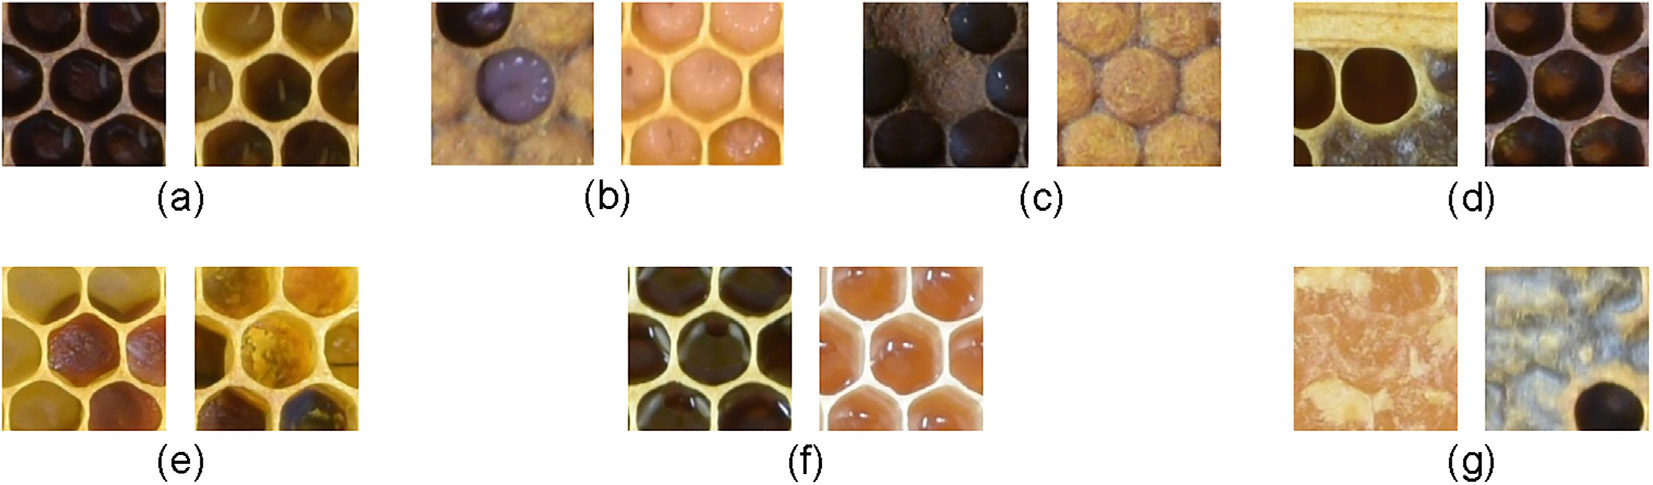
\includegraphics[width=\textwidth]{./images/deepbee-cell-classes.jpg}
	\caption{Exemple vizuale de clase de celule de fagure folosite în articolul DeepBee pentru clasificarea automată. Imagine preluată din articolul \cite{deepbeeArticle}.}
	\label{fig:deepbee-clase-celule}
\end{figure}

Pornind de la aceste exemple vizuale (figura~\ref{fig:deepbee-clase-celule}), fluxul conceptual al clasificării poate fi rezumat printr-o succesiune de pași: pregătirea regiunii de imagine, extragerea caracteristicilor prin straturi convoluționale și transformarea rezultatului în probabilități pentru clasele relevante. Acest flux este ilustrat în figura~\ref{fig:flux-cnn-celule-fagure}.

\begin{figure}[H]
	\centering
	\resizebox{\textwidth}{!}{%
	\begin{tikzpicture}[
		layer/.style={draw, rounded corners=3pt, fill=gray!8, minimum height=1.05cm, text width=2.45cm, align=center, font=\small},
		process/.style={draw, rounded corners=3pt, fill=yellow!15, minimum height=1.05cm, text width=2.45cm, align=center, font=\small},
		output/.style={draw, rounded corners=3pt, fill=green!10, minimum height=1.05cm, text width=2.85cm, align=center, font=\small},
		arrow/.style={-{Latex[length=2mm]}, thick}
	]
		\node[layer] (input) {Crop celulă\\224 x 224 x 3};
		\node[process, right=0.55cm of input] (prep) {Preprocesare\\normalizare Keras};
		\node[layer, right=0.55cm of prep] (conv1) {Convoluții\\filtre locale};
		\node[layer, right=0.55cm of conv1] (pool1) {Pooling\\reducere spațială};
		\node[layer, right=0.55cm of pool1] (features) {Blocuri CNN\\caracteristici profunde};
		\node[layer, right=0.55cm of features] (classifier) {Strat dens\\clasificator};
		\node[output, right=0.55cm of classifier] (softmax) {Softmax\\probabilități pe clase};

		\node[output, below=1.05cm of softmax] (classes) {\texttt{Capped}, \texttt{Eggs}, \texttt{Honey}\\\texttt{Larves}, \texttt{Nectar}, \texttt{Other}, \texttt{Pollen}};
		\node[process, below=1.05cm of features] (quality) {Scor de încredere\\metadată de calitate};

		\draw[arrow] (input) -- (prep);
		\draw[arrow] (prep) -- (conv1);
		\draw[arrow] (conv1) -- (pool1);
		\draw[arrow] (pool1) -- (features);
		\draw[arrow] (features) -- (classifier);
		\draw[arrow] (classifier) -- (softmax);
		\draw[arrow] (softmax) -- (classes);
		\draw[arrow] (softmax.south west) -- (quality.north east);
	\end{tikzpicture}}
	\caption{Fluxul datelor printr-o rețea neuronală convoluțională folosită pentru clasificarea celulelor de fagure. Schema prezintă nivelul conceptual al inferenței, nu arhitectura internă completă a modelului DeepBee.}
	\label{fig:flux-cnn-celule-fagure}
\end{figure}

Clasificarea este executată în loturi de celule. În configurația Azure folosită pentru testarea pe telefon, lotul de clasificare are 64 de crop-uri. Această decizie nu schimbă modelul și nu reduce numărul de celule analizate; schimbă doar modul de inferență, astfel încât serviciul să nu țină simultan în memorie toate regiunile 224 x 224 extrase dintr-o ramă densă.

Acest mod de lucru are avantaje și limite. Avantajul este că transformă o fotografie complexă într-o sumă de decizii locale. Limita este că modelul vede fiecare regiune într-un context restrâns. Informații precum distribuția spațială a puietului, compactitatea reală a ramei sau pattern-ul bolilor pot necesita date suplimentare sau modele care păstrează coordonatele celulelor. În BeeSmart, indicatorii calculați din numărători sunt utili, dar nu trebuie interpretați ca diagnostic complet.

\section{MobileNet și eficiența procesării}

Articolul DeepBee compară mai multe arhitecturi și discută raportul dintre acuratețe și timp de procesare \cite{deepbeeArticle}. Într-o aplicație practică, nu este suficient ca modelul să fie precis; el trebuie să fie suficient de rapid pentru a fi folosit în fluxul normal al utilizatorului. Dacă analiza unei fotografii durează prea mult, utilizatorul va evita funcția sau o va percepe ca pe un blocaj.

MobileNet este o familie de arhitecturi CNN proiectate pentru eficiență pe dispozitive mobile și în contexte cu resurse limitate \cite{mobilenetHoward2017}. Ideea principală este reducerea costului computațional prin convoluții separabile în adâncime (\emph{depthwise separable convolutions}), care descompun o convoluție standard în două operații mai simple: o convoluție pe adâncime, aplicată independent fiecărui canal, și o convoluție punctuală $1 \times 1$, care combină rezultatele între canale.

Beneficiul poate fi cuantificat. Pentru o intrare cu $M$ canale, un strat de ieșire cu $N$ canale, nuclee de dimensiune $D_K \times D_K$ și o hartă de caracteristici de dimensiune $D_F \times D_F$, costul unei convoluții standard este
\begin{equation}
	C_{\text{std}} = D_K \cdot D_K \cdot M \cdot N \cdot D_F \cdot D_F,
	\label{eq:cost-std}
\end{equation}
în timp ce costul variantei separabile în adâncime este
\begin{equation}
	C_{\text{dws}} = D_K \cdot D_K \cdot M \cdot D_F \cdot D_F + M \cdot N \cdot D_F \cdot D_F.
	\label{eq:cost-dws}
\end{equation}
Raportul dintre cele două costuri arată reducerea obținută:
\begin{equation}
	\frac{C_{\text{dws}}}{C_{\text{std}}} = \frac{1}{N} + \frac{1}{D_K^2}.
	\label{eq:cost-ratio}
\end{equation}
Pentru nuclee uzuale de $3 \times 3$ ($D_K = 3$) și un număr mare de canale de ieșire, factorul $1/N$ devine neglijabil, iar reducerea de cost se apropie de $1/D_K^2 \approx 1/9$, adică un cost de aproximativ opt-nouă ori mai mic, cu o pierdere mică de acuratețe. Aceste arhitecturi urmăresc, așadar, să păstreze performanța de clasificare cu semnificativ mai puține operații decât rețelele convoluționale mari.

Pentru BeeSmart, relevanța MobileNet este dublă. Pe de o parte, DeepBee indică importanța unui model eficient pentru clasificarea celulelor. Pe de altă parte, chiar dacă modelul rulează pe server și nu direct pe telefon, timpul de procesare rămâne important. Serviciul AI trebuie să răspundă suficient de rapid pentru ca formularul de inspecție să rămână utilizabil. Eficiența nu este doar o problemă de cost server, ci și una de experiență a utilizatorului.

În implementarea curentă, această idee este aplicată și la nivel de infrastructură. Clientul Android păstrează fotografia de inspecție la o calitate suficient de mare pentru arhivare, dar trimite către endpoint-ul AI o versiune redimensionată și comprimată special pentru analiză. În serviciul Python, modelul de segmentare DeepBee este aplicat pe patch-uri, imaginea nu mai este mărită obligatoriu la 6000 x 4000 pixeli pentru fiecare cerere, iar clasificarea este executată în batch-uri. Astfel se păstrează rolul teoretic al segmentării și clasificării din DeepBee, dar timpul de răspuns și consumul de memorie devin compatibile cu testarea pe telefon și cu rularea în Azure Container Apps.

\section{Indicatori derivați din rezultatele AI}

Rezultatul brut al serviciului AI este o corespondență între clasă și număr de celule. Pentru utilizator, acest rezultat trebuie transformat într-o formă interpretabilă. De exemplu, un dicționar care spune că au fost detectate 30 de celule de larve și 80 de celule de puiet căpăcit este util, dar devine mai clar dacă aplicația calculează proporții, densități și tendințe.

În BeeSmart, transformarea se face atât pe client, cât și pe backend. Pe Android, \path{BroodAnalyzer} agregă clasele în categorii stabile și calculează indicatori precum totalul de puiet, raportul larve/puiet căpăcit, raportul rezervelor și o estimare orientativă a compactității. Pe backend, \path{InspectionService} normalizează rezultatele și salvează indicatori precum totalul de celule, celule de puiet, celule de rezerve, densitatea puietului și raportul rezervelor.

Acești indicatori trebuie prezentați ca suport decizional. Ei pot sugera că există puiet, că rezervele sunt scăzute sau că raportul dintre larve și puiet căpăcit merită verificat. Totuși, ei nu confirmă boli și nu înlocuiesc controlul fizic al ramei. Calitatea fotografiei, calitatea detecției și domeniul pe care a fost antrenat modelul influențează rezultatul.

\section{Calitatea fotografiei și utilizarea în teren}

Un sistem de analiză vizuală este sensibil la calitatea imaginii. O fotografie neclară, întunecată, supraexpusă, făcută din unghi sau acoperită parțial de albine poate produce rezultate înșelătoare. Din acest motiv, BeeSmart verifică dimensiunea imaginii, claritatea, luminozitatea, contrastul, numărul de celule detectate și raportul predicțiilor cu încredere scăzută.

Statusurile precum \path{low_quality} sau \path{uncertain_analysis} sunt importante atât tehnic, cât și pentru experiența utilizatorului. Într-o stupină, aplicația trebuie să răspundă clar și să nu blocheze formularul principal dacă analiza AI eșuează. Un mesaj de refotografiere este mai util decât o distribuție de clase calculată pe o imagine nepotrivită, iar rezultatul trebuie prezentat ca informație de sprijin, nu ca verdict absolut.

\section{Integrarea modelului AI într-un flux software}

Integrarea AI într-o aplicație nu înseamnă doar apelarea unui model. Este necesar un flux complet: captarea fotografiei, transmiterea ei, validarea payload-ului, procesarea, tratarea erorilor, salvarea rezultatului și afișarea într-o formă inteligibilă. În BeeSmart, utilizatorul adaugă o fotografie în Android, clientul trimite versiunea optimizată către backend, backend-ul validează cererea, serviciul AI procesează imaginea, iar rezultatul se întoarce în aplicație.

Backend-ul are un rol de protecție între client și serviciul AI: respinge imaginile Base64 invalide, tratează răspunsurile incorecte și întoarce erori HTTP controlate când serviciul AI nu răspunde. Tot backend-ul leagă rezultatul de inspecție, stup și stupină, astfel încât analiza să devină parte din istoricul apicol, nu doar un răspuns izolat.

Răspunsul serviciului AI include și metadate de calitate, nu doar numărătorile finale. Printre acestea se află dimensiunile imaginii, dimensiunea payload-ului, numărul de celule detectate și clasificate, media încrederii, raportul predicțiilor slabe, numărul de patch-uri de segmentare și timpii principalelor etape. Aceste informații au fost utile în stabilizarea deployment-ului Azure și pot susține mesaje mai bune atunci când analiza nu este sigură.

\section{Responsabilitatea interpretării rezultatelor AI}

Orice funcție AI dintr-o aplicație practică trebuie prezentată cu responsabilitate. În domeniul apicol, un rezultat automat poate ajuta la observarea unor semnale, dar nu poate înlocui experiența apicultorului sau evaluarea unui specialist. BeeSmart trebuie să evite formulările care ar sugera diagnostic veterinar cert; un raport despre celule detectate și proporții poate susține decizia, dar nu o poate lua în locul utilizatorului.

Această delimitare este importantă și pentru corectitudine academică. Interfața nu trebuie să ascundă incertitudinea, iar tendințele trebuie descrise ca evoluții observate în date, nu ca predicții medicale. Contribuția proiectului este integrarea unor rezultate automate într-un sistem de evidență, nu certificarea clinică a unei familii de albine.

\section{Legătura dintre suportul teoretic și BeeSmart}

Suportul teoretic prezentat în acest capitol se reflectă direct în aplicație. Trasabilitatea explică păstrarea istoricului, offline-first explică baza Room și coada de sincronizare, consistența eventuală explică rezolvarea identificatorilor locali, iar securitatea explică folosirea JWT și verificările de ownership.

În partea AI, DeepBee explică împărțirea analizei în detecție, segmentare și clasificare. Hough Circle Transform localizează celulele candidate, rețelele convoluționale clasifică regiunile, iar MobileNet justifică atenția acordată raportului dintre acuratețe și timp de procesare. Indicatorii derivați transformă rezultatul brut într-o formă utilă pentru utilizator.

Prin urmare, BeeSmart nu este doar o colecție de biblioteci software. Fiecare tehnologie și fiecare concept susține o nevoie funcțională: lucru în teren, date structurate, sincronizare, securitate, analiză vizuală și interpretare prudentă. Această legătură dintre domeniu, teorie și implementare este fundamentul capitolelor următoare ale lucrării.
